
%%%%%%%%%%%%%%%%%%%%%%%%%%%%%%%%%%%%%%%%%%%%%%%%%%%%%%%%%%
\chapter{Related Work}
\label{chapter_related_work}
%%%%%%%%%%%%%%%%%%%%%%%%%%%%%%%%%%%%%%%%%%%%%%%%%%%%%%%%%%

\begin{figure}
\centering
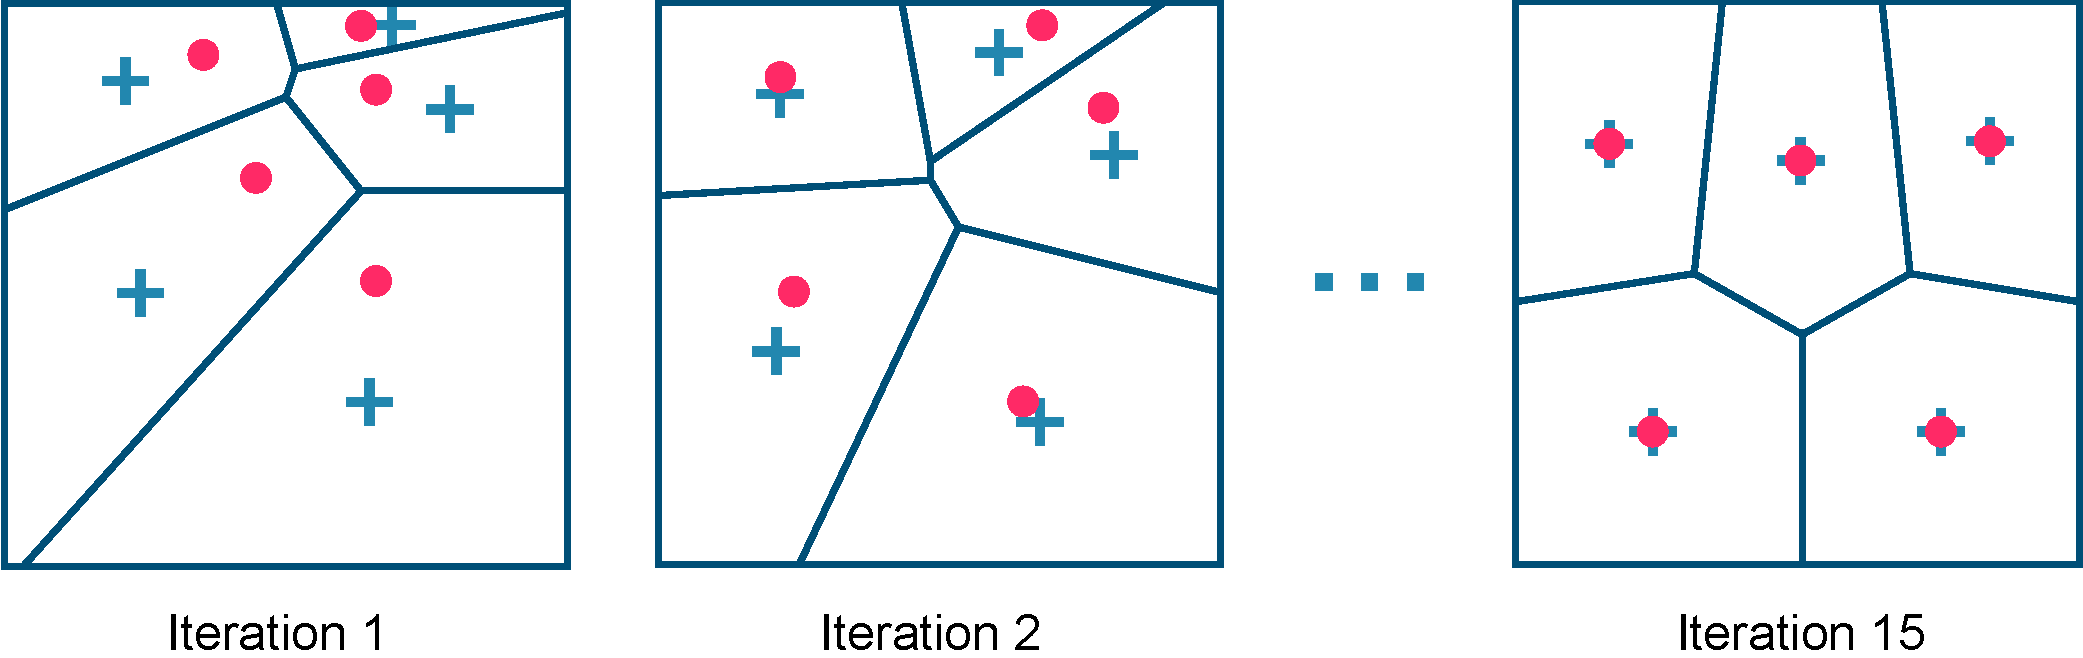
\includegraphics[width=1.0\textwidth]{figures/related/lloyds_method.pdf} 
\caption[An illustration of Lloyd's method.]
{\label{fig_lloyds_method} 
\newtext
{
An illustration of Lloyd's method.
A Voronoi diagram is generated from the input point elements (drawn as red dots).
We then move the point elements to the centroids of Voronoi cells (drawn as plus signs).
The process is repeated until convergence, producing a centroidal Voronoi diagram.
Figure source is Wikipedia, drawn by Dominik Moritz under CC0 1.0.
}
}
\end{figure}


\begin{figure}
\centering
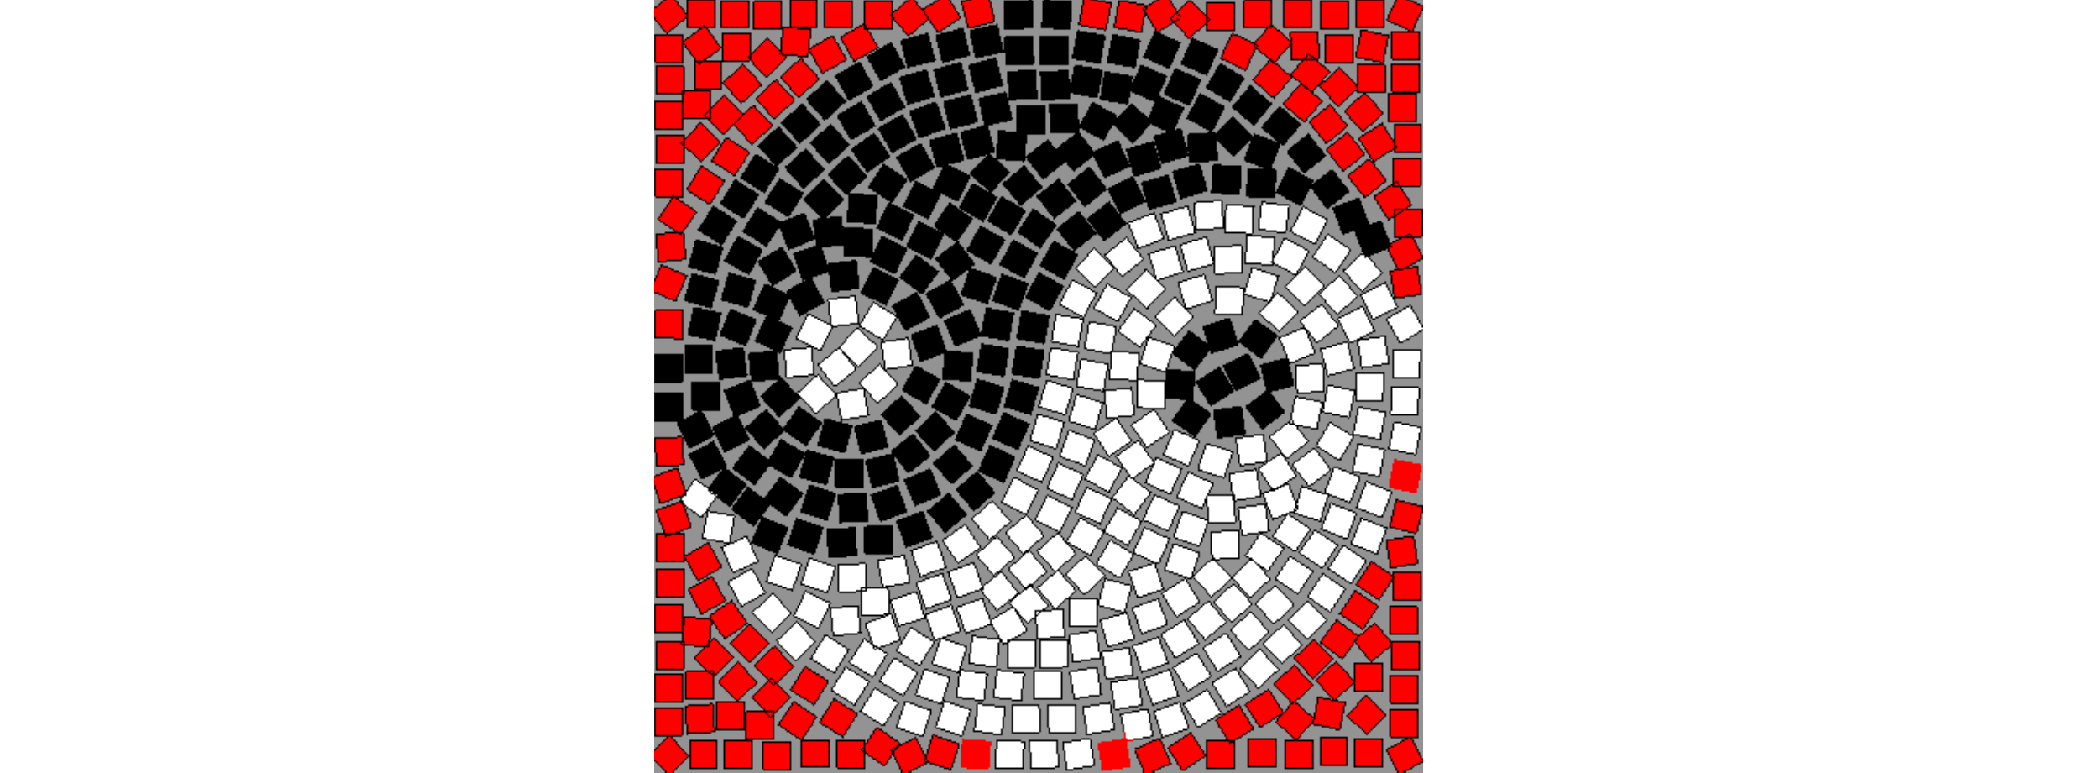
\includegraphics[width=1.0\textwidth]{figures/related/hausner.pdf} 
\caption[Decorative mosaics using Lloyd's method]
{\label{fig_related_hausner} 
\newtext
{
Mosaics of square elements generated using Lloyd's method with Manhattan distance~\cite{Hausner2001}
}
}
\end{figure}





%%%%%%%%%%%%%%%%%%%%%%%%%%%%%%%%%%%%%%%%%%%%%%%%%%%%%%%%%%
\section{2D Packings}
%%%%%%%%%%%%%%%%%%%%%%%%%%%%%%%%%%%%%%%%%%%%%%%%%%%%%%%%%%

%Rigid packing algorithms attempt to distribute elements through rigid transformations.
%These algorithms can be categorized into two groups: iterative methods and data-driven methods.
%Iterative methods start with an initial configuration then they use a variant of Lloyd's method 
%to refine the configuration to an even distribution of elements.
%data-driven methods rely on a shape matching algorithm to find a matching element from
%an element library.
%Some of rigid packing algorithms have an additional step where they 
%correct gaps and overlaps using deformation, the deformation was applied
%locally near edges in a post-processing step after elements
%were frozen in place.

\newtext
{
\textbf{Lloyd's Method:}
An approach to generate a packing is to start with an initial configuration and iteratively refine it using Lloyd's method
to obtain an even distribution of elements. 
Figure~\ref{fig_lloyds_method} shows an illustration of the simplest example of 
Lloyd's method that distributes point elements.
Given $N$ point elements, 
we first compute a \textit{Voronoi diagram} to partition the plane into $N$ regions such that
all points inside a Voronoi cell are closest to its associated point element.
As an iterative process, 
the Lloyd's method moves every point elements to the centroid of its Voronoi cell, 
then the Voronoi diagram is recomputed.
The process is repeated until the distribution is even,
that means all the point elements are located at the the centroids of the Voronoi cells.
The final structure is called a \textit{Centroidal Voronoi Diagram} (CVD).
}

\newtext
{
Hausner~\cite{Hausner2001} modified the Lloyd's method to distribute square elements into a container 
region, simulating the appearance of traditional mosaics (Figure~\ref{fig_related_hausner}). 
This can be achieved by replacing Euclidean distance with Manhattan distance so that Voronoi cells resemble squares instead of hexagons.
It turns out that a customized distance function can be used to manipulate the shapes of Voronoi cells.
%we will discuss a few more of related work that use this exploit throughout this chapter. 
However, Hausner's approach can only translate the squares, and a vector field is required to rotate them.
Furthermore, more complicated shapes such as long rectangles would have severe overlaps.
More recently, Javid et al.~\cite{Javid2019} constructed a distance function that 
incorporates a spatial distance, a color distance, and an elongation factor. Their resulted
Voronoi cells have elongated shapes, resembling pebble-like mosaics.
}

\newtext
{
Hiller et al.~\cite{Hiller2003} improved upon the Lloyd's method to generate \textit{Centroidal Area Voronoi Diagram} (CAVD),
a variant of CVD that is a distribution of simple polygonal elements.
This new extension computes the main inertia axis for each Voronoi cell so that 
its element can be rotated to get better alignment with the Voronoi cell boundary.
In follow up work, Smith et al.~\cite{Smith2005} generated temporally coherent animated mosaics by utilizing CAVD.
Dalal et al.~\cite{Dalal2006} used an FFT-based image correlation to reposition
and rotate elements with their Voronoi cell boundaries, which could be seen as making more effective use of negative
space, and permitting non-convex elements to interlock more than they did in
earlier methods.
}

\newtext
{
\textbf{Data-Driven Method:} 
A different approach to generate packings is to use a shape matching algorithm
and it requires a library containing a large number of elements (Figure~\ref{fig_related_jim_pad}).
This is usually done by placing an element one by one until the container area is filled.
For each step, a shape matching algorithm selects an 
element that has the best fit with the previously placed elements or the container boundary.
Jigsaw Image Mosaics~\cite{Kim2002} used a geometric hashing to find
a compatible element. JIM places elements using a greedy approach, but is able to backtrack 
if previous configuration is more optimal.
Pyramid of Arclength Descriptor~\cite{Kwan2016} developed
a partial shape matching algorithm that can match a subset of element boundary with a portion
of container boundary.
}

\newtext
{
It is also possible to initially partition the container into smaller segments
and independently replace each segment with a matching element.
This is desirable if the container has colors or salient parts that need to be preserved.
Huang et al.~\cite{Huang2011} produced Arcimboldo-like collages
by arranging cutout images collected from the internet.
Their container is a larger cutout image which is partitioned into segments
using an image segmentation algorithm.
Each segment is then replaced with a smaller cutout image that has a similar shape and color.
}

\newtext
{
All these data-driven methods require an element library that is big enough,
the more elements in the library will increase their chance to find a compatible element boundary.
However, bigger database means increased computational time.
Collecting a large number of elements is also not always feasible,
for example, if an artist wants to create a packing of a hand-drawn cats,
they may not want to draw 1000 cats which is tedious and repetitive.
}

\begin{figure}
\centering
\includegraphics[width=1.0\textwidth]{figures/related/jim_pad.pdf} 
\caption[Examples of packings generated by JIM and PAD]
{\label{fig_related_jim_pad} 
\newtext
{
Data-driven methods:
(a) Jigsaw Image Mosaics~\cite{Kim2002}.
(b) Pyramid of Arclength Descriptor~\cite{Kwan2016}. 
}
}
\end{figure}




\begin{figure}
\centering
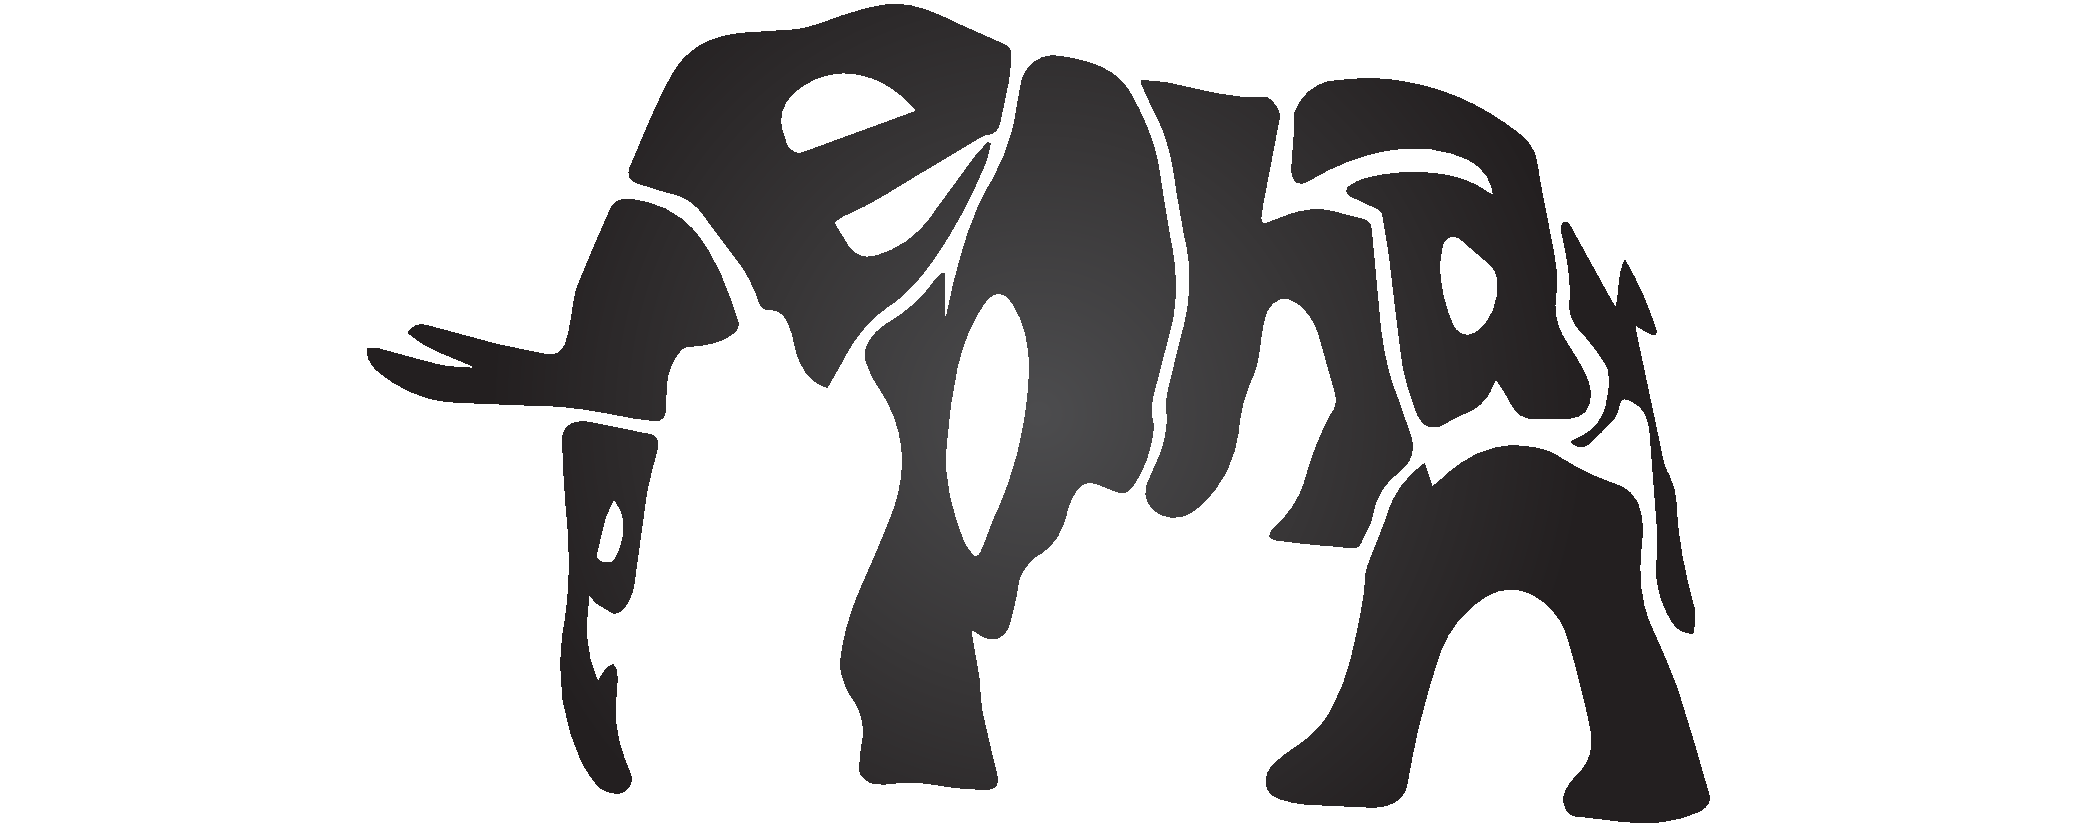
\includegraphics[width=1.0\textwidth]{figures/related/calligraphy.pdf} 
\caption[A calligraphy packing of an ``elephant'']
{\label{fig_calligraphy_packing} 
\newtext
{
A deformation-driven packing of a calligraphic ``elephant''~\cite{Xu2007}.
}
}
\end{figure}

%%%%%%%%%%%%%%%%%%%%%%%%%%%%%%%%%%%%%%%%%%%%%%%%%%%%%%%%%%
%\section{Non-rigid Packing Methods}
%%%%%%%%%%%%%%%%%%%%%%%%%%%%%%%%%%%%%%%%%%%%%%%%%%%%%%%%%%

% need to consult to FLOWPAK for variety
\newtext
{
\textbf{Deformation-Driven Method:}
Instead of finding compatible elements,
a deformation-driven method forces elements to create compatibilities and shape variations.
As an advantage, a deformation-driven method can rely on a small size element library.
Peng et al.~\cite{Peng2014} computed layouts by packing and deforming
simple polygons and polyominoes, although their method cannot handle more
complicated shapes.
Xu and Kaplan~\cite{Xu2007} and Zou et al.~\cite{Zou2016}
constructed \textit{calligrams} by filling a container with a small
number of deformed letters composing one or two words (Figure~\ref{fig_calligraphy_packing}).  
Their goal was to balance between filling the container and preserving readability.
Abdrashitov et al.~\cite{Abdrashitov2014} developed
a sketch-based interface where an artist can draw curves where square-like elements are placed along it
create a mosaic arrangement.
After the square elements are frozen in place, 
they are deformed to eliminate overlap, to create shape variations, 
and to even even out the negative space.  
}
%Zehnder et al.~\cite{Zehnder2016} proposed an method to
%cover 3D surfaces with deformed ornamental elastic curves.

%Some of rigid packing algorithms have an additional step where they 
%correct gaps and overlaps using deformation, the deformation was applied
%locally near edges in a post-processing step after elements
%were frozen in place.

\begin{figure}
\centering
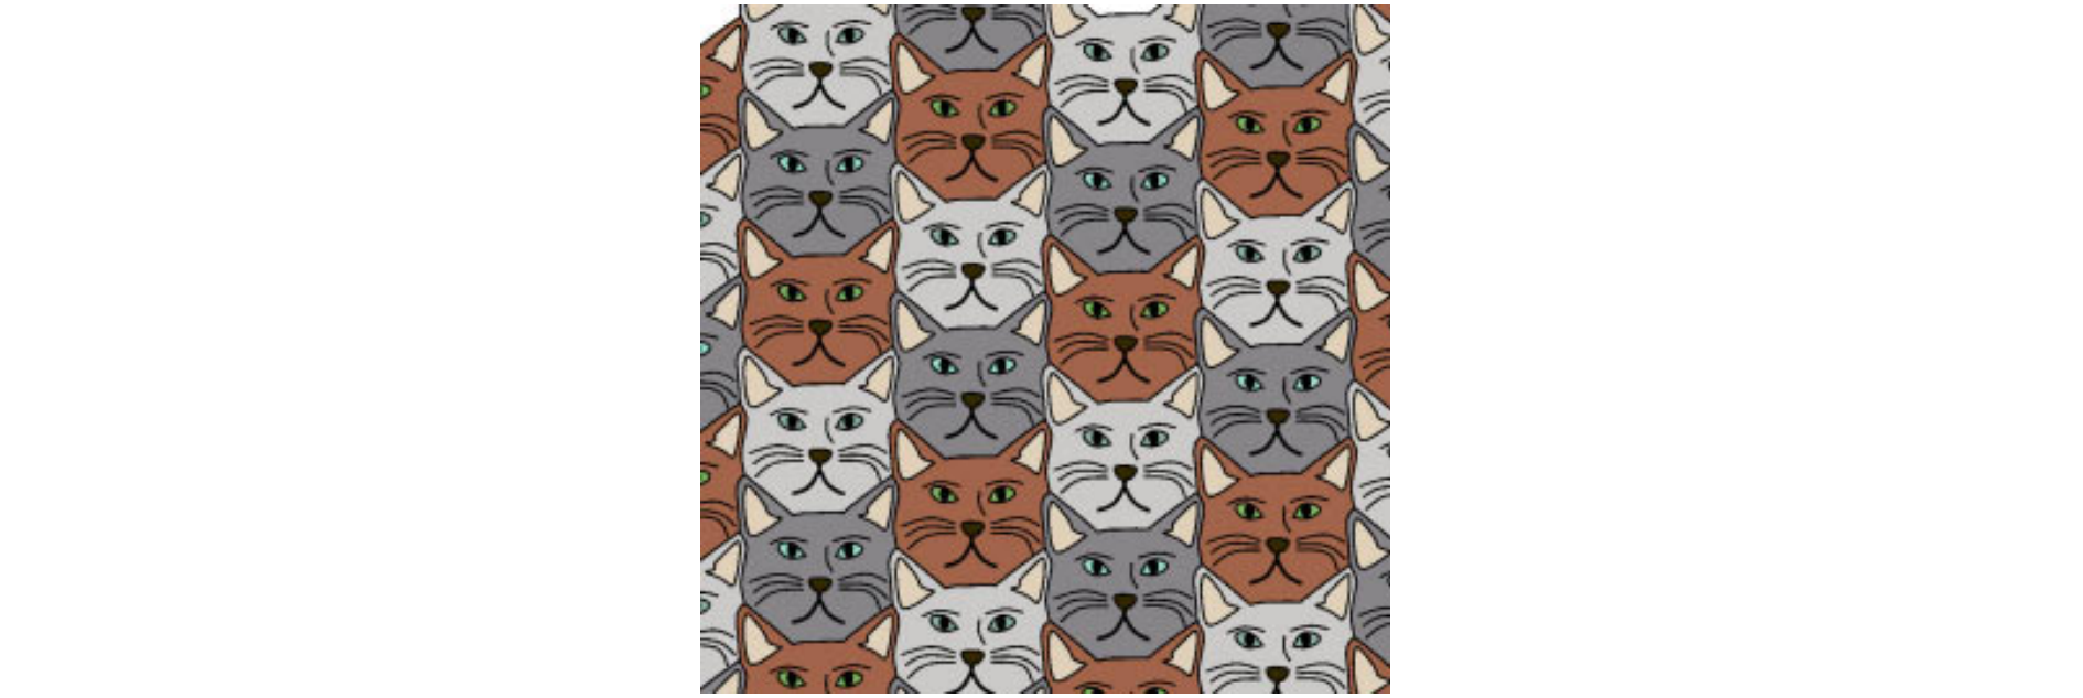
\includegraphics[width=1.0\textwidth]{figures/related/escherization.pdf} 
\caption[An example of a tiling]
{\label{fig_related_escherization} 
\newtext
{
A tiling of cats~\cite{Kaplan2000}. 
}
}
\end{figure}

%%%%%%%%%%%%%%%%%%%%%%%%%%%%%%%%%%%%%%%%%%%%%%%%%%%%%%%%%%
\section{Tilings}
%%%%%%%%%%%%%%%%%%%%%%%%%%%%%%%%%%%%%%%%%%%%%%%%%%%%%%%%%%

\newtext
{
As elements reach perfect compatibility, a packing turns to a tiling, see Figure~\ref{fig_related_escherization} for an example.
The element boundaries interlock, leaving no negative space.
Kaplan and Salesin~\cite{Kaplan2000, Kaplan2004} deformed one or two 
input elements into ones that can tile the plane.
Given an input element $E$ they look for a similar tile $T$
from a parameterized tiling space.
Due to high frequency deformations,
$T$ is often perceptually unrecognizable from its silhouette unless an interior picture is added.
They can fail to find $T$ if $E$ has deep concavity, for example, a ``G'' shape.
The tile $T$ also cannot fill a container due to its highly structured boundary.
}

\newtext
{
Lin et al.~\cite{Lin2018} generated tiling arrangements that resemble Escher's Sky and Water I.
Two original elements $S_1$ and $S_2$ are placed on the opposite sides of a rectangular canvas,
 they are then copied and arranged in rows such 
that the copies in the middle of canvas tile each other.
%Two original elements $S_1$ and $S_2$ are placed on the opposite sides of a rectangular canvas.
%Then copies of each element are spread away in rows, 
%until they meet and tile each other right in the middle of the canvas.
The farther a copy from the original element, the more deformed it is, 
creating a ``fading effect'', $S_1$ and $S_2$ spatially transition to negative space.
This work is data-driven, the user needs to provide $S_1$, 
and the method tries to find a compatible element $S_2$ from a library.
}

%%%%%%%%%%%%%%%%%%%%%%%%%%%%%%%%%%%%%%%%%%%%%%%%%%%%%%%%%%
\section{Discrete Texture Synthesis}
%%%%%%%%%%%%%%%%%%%%%%%%%%%%%%%%%%%%%%%%%%%%%%%%%%%%%%%%%%

\newtext
{
Some past work has sought to adapt example-based texture synthesis methods
from raster images to vector graphics, producing distributions of
rigidly transformed elements that mimic the statistics of an exemplar.
An element is represented as a single point, which is adequate for a small rigid element.
Barla et al.~\cite{Barla2006} and Ijiri et al.~\cite{Ijiri2008} used a growth model that copies small neighbourhoods
from the exemplar into a larger output texture.  AlMeraj et al.~\cite{AlMeraj2013}
stamped out copies of the exemplar and discard overlapping elements.
Hurtut et al.~\cite{Hurtut2009} developed a statistical sampling method based
on multitype point processes.  
Loi et al.~\cite{Loi2017} developed a texture synthesis method that
can specify global arrangements, local arrangements, or a blend of multiple arrangements.
These techniques are all concerned with replicating
the uneven element distribution in the exemplar, without regard for negative space.
}

\newtext
{
For more complex elements, a single point representation is not enough.
Ma et al.~\cite{Ma2011} used sample-based representation 
that works by distributing a sparse set of points inside an element.
They later distributed these points using a neighborhood metric and an iterative optimization.
Unlike previous work, they are able synthesize textures with long deformable elements, for example, spaghetti.
Ma et al. later extended their work to accept animated elements~\cite{Ma2013}, where
a sample point has spatial and time positions, turning the problem to spacetime texture synthesis.
More recently, Hsu et al.~\cite{Hsu2020} adapted the sample-based representation into a user interface
where an artist can initially distribute elements by drawing strokes
which are then optimized using a Lloyd-like optimization.
}
%Most discrete texture synthesis method treat a single element
%Ma et al.~\cite{Ma2011} used sample-based element representation 
%Ma et al.~\cite{Ma2011} use sparse point samples to represent an element, which
%give an advantage of distributing 




%%%%%%%%%%%%%%%%%%%%%%%%%%%%%%%%%%%%%%%%%%%%%%%%%%%%%%%%%%
\section{3D Packings}
%%%%%%%%%%%%%%%%%%%%%%%%%%%%%%%%%%%%%%%%%%%%%%%%%%%%%%%%%%
\newtext
{
Collages are arragements of overlapping elements, similar to
portrait paintings by Arcimboldo.
Gal et al.~\cite{Gal2007B} presented a method for constructing 3D
collages (Figure~\ref{fig_related_gal_zehnder}a).  They filled a 3D container with overlapping 3D elements using a greedy
approach and a partial shape matching algorithm.
Huang et al.~\cite{Huang2014} designed a method
to generate mechanical collages, such as giant robots.
Theobalt et al.~\cite{Theobalt2007}
developed a method to generate animated 3D collages.
They segment an animated container
into smaller rigid parts, each is replaced with a matching element.
The final result of animated collage consists of rigid motions of elements.
All these collage methods require a 3D shape database so they are considered as data-driven. 
%Both these collage methods require a 3D shape database so they can be considered as data-driven. 
}

\newtext
{
The cutting and packing problem (C\&P) is defined as cutting a large object into smaller parts 
which are then packed inside a container.
C\&P is popular in manufacturing and 3D printing because
objects can be produced with less waste material and packed into a smaller box.
A good cutting process is critical in C\&P, if it can decompose the input object
into simpler parts, then the packing process can be easier.
Chernov et al.~\cite{Chernov2010} proposed a method to decompose a large object
into smaller phi objects which can be packed more efficiently.
They define a phi object as a shape whose surface boundaries 
are flat, spherical, cylindrical, or conical.
Vanek et al.~\cite{Vanek2014} introduced PackMerger,
a method to pack thin shells which can be assembled together into
a larger watertight object.
In follow up work, Chen et al.~\cite{Chen2015} introduced Dapper,
a method to cut and pack volumetric printed objects.
}

\newtext
{
In engineering, packings are useful for a number of applications, 
such as product packaging, circuit designs, or mechanical layouts.
Packing of irregular rigid 3D elements without overlaps 
is a still challenging research topic.
Byholm et al.~\cite{Byholm2009} developed a method
to pack voxelized elements, which are easier for collision detection.
Ma et al.~\cite{Ma2018} developed a heuristic method
to pack triangular meshes.
For an in-depth survey, Cagan et al.~\cite{Cagan2002} discussed a few approaches such as
gradient methods, heuristics, simulated annealing, and genetic algorithms.
}



%%%%%%%%%%%%%%%%%%%%%%%%%%%%%%%%%%%%%%%%%%%%%%%%%%%%%%%%%%
\section{Packings on Surfaces}
%%%%%%%%%%%%%%%%%%%%%%%%%%%%%%%%%%%%%%%%%%%%%%%%%%%%%%%%%%

\newtext
{
Some recent work has explored the elaboration of ornamental
patterns on surfaces, under constraints imposed by fabrication.  
Chen et al.~\cite{Chen2016} developed a method to generate a filigree pattern,
which is an arrangement of decorative thin rod elements on a surface.
Given an initial random configuration of overlapping elements, their method
removes overlaps by either deforming or trimming the rods.
Bian et al.~\cite{Bian2018} used Wang tiles made of element parts to generate filigree patterns.
In similar work, Zehnder et al.~\cite{Zehnder2016} 
proposed a semi-automated tool for deforming ornamental curves to cover a surface (Figure~\ref{fig_related_gal_zehnder}b). 
They start with an initial configuration of scaled down elements
that has no overlaps. They later extend the rod elements and 
overlaps can be avoided by deforming the rods.
Mart\'{\i}nez et al.~\cite{Martinez2019} developed a method to generate
star-shaped tiling patterns that are printed onto tracery sheets.
Similar to Hausner's exploit, their method works by constructing a star-shaped distance function to manipulate the shapes of Voronoi cells. 
}

\makeatletter % brooo
\setlength{\@fptop}{0pt} % brooo
\makeatother % brooo
\begin{figure}[ht!]
\centering
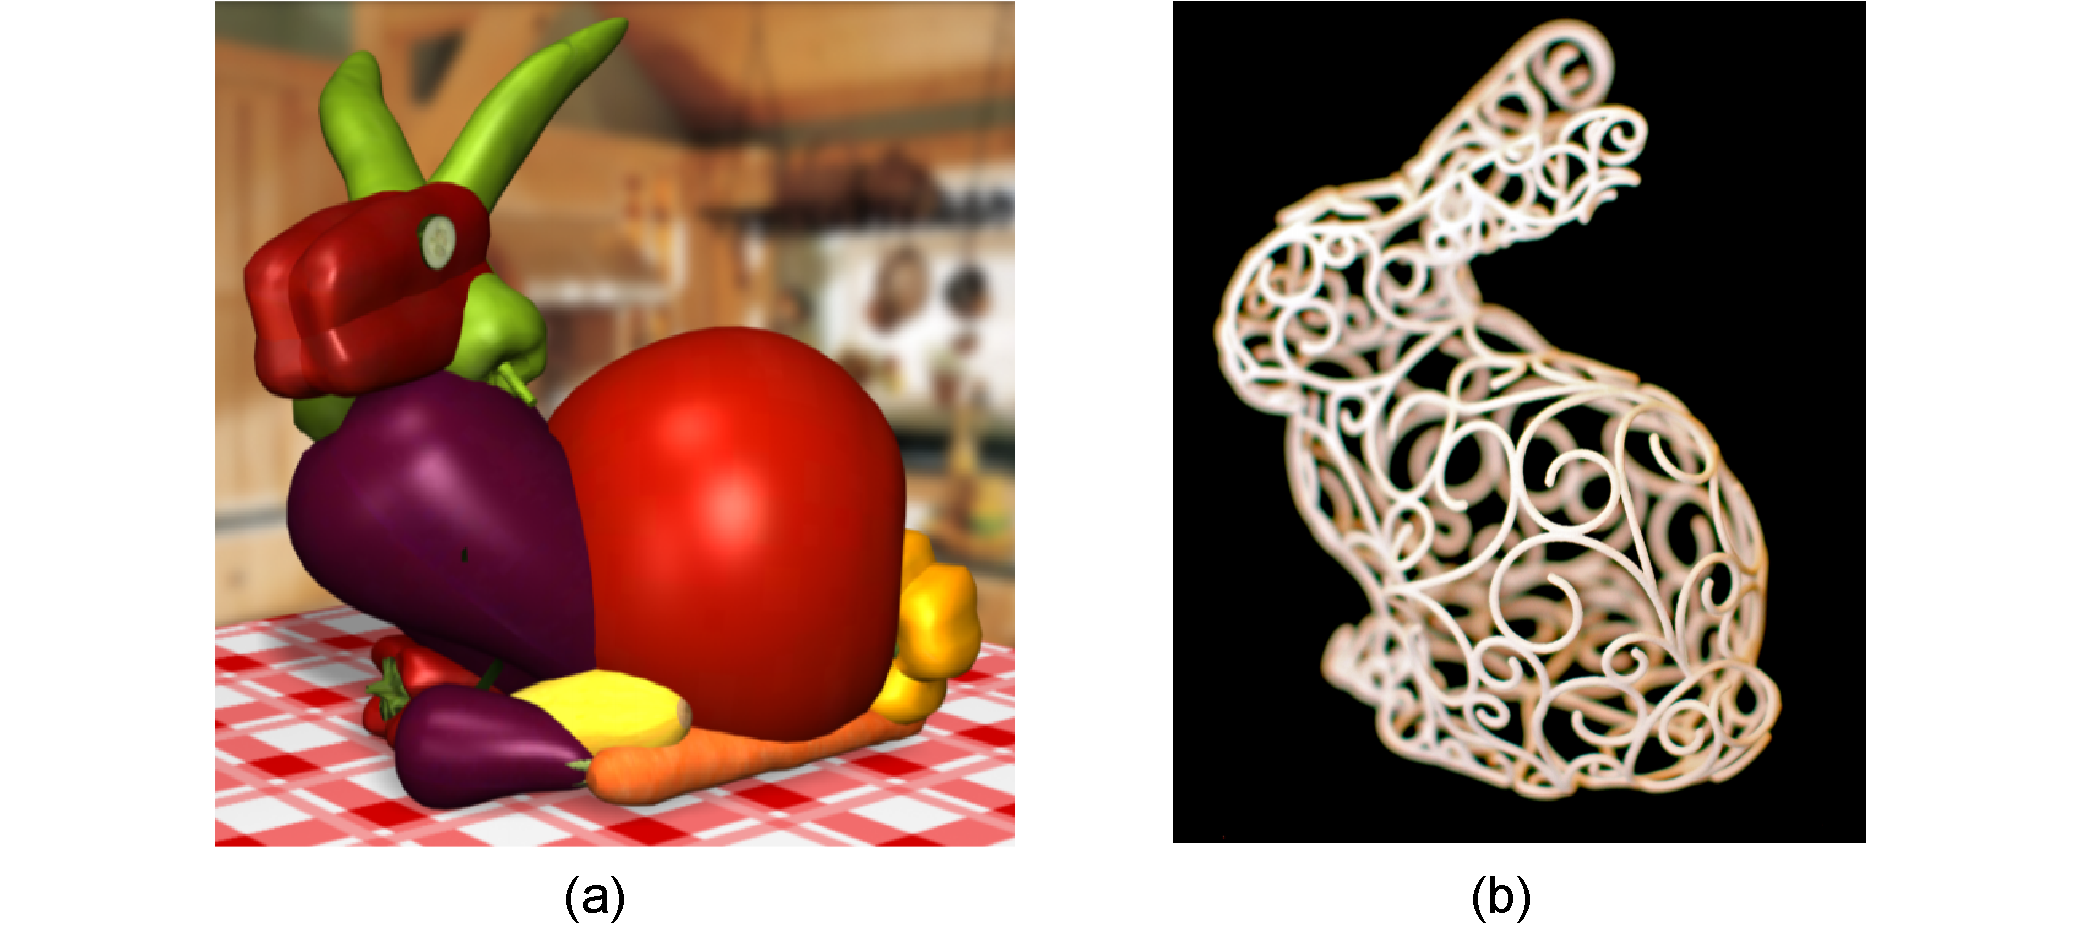
\includegraphics[width=1.0\textwidth]{figures/related/gal_zehnder.pdf} 
\caption[An example of decorative ornaments filling a surface]
{\label{fig_related_gal_zehnder} 
\newtext
{
(a) Arcimboldo-like 3D packing~\cite{Gal2007B}. 
(b) Decorative elements that fill a surface~\cite{Zehnder2016}.
}
}
\end{figure}